% Options for packages loaded elsewhere
\PassOptionsToPackage{unicode}{hyperref}
\PassOptionsToPackage{hyphens}{url}
%
\documentclass[
]{article}
\usepackage{amsmath,amssymb}
\usepackage{iftex}
\ifPDFTeX
  \usepackage[T1]{fontenc}
  \usepackage[utf8]{inputenc}
  \usepackage{textcomp} % provide euro and other symbols
\else % if luatex or xetex
  \usepackage{unicode-math} % this also loads fontspec
  \defaultfontfeatures{Scale=MatchLowercase}
  \defaultfontfeatures[\rmfamily]{Ligatures=TeX,Scale=1}
\fi
\usepackage{lmodern}
\ifPDFTeX\else
  % xetex/luatex font selection
\fi
% Use upquote if available, for straight quotes in verbatim environments
\IfFileExists{upquote.sty}{\usepackage{upquote}}{}
\IfFileExists{microtype.sty}{% use microtype if available
  \usepackage[]{microtype}
  \UseMicrotypeSet[protrusion]{basicmath} % disable protrusion for tt fonts
}{}
\makeatletter
\@ifundefined{KOMAClassName}{% if non-KOMA class
  \IfFileExists{parskip.sty}{%
    \usepackage{parskip}
  }{% else
    \setlength{\parindent}{0pt}
    \setlength{\parskip}{6pt plus 2pt minus 1pt}}
}{% if KOMA class
  \KOMAoptions{parskip=half}}
\makeatother
\usepackage{xcolor}
\usepackage[margin=1in]{geometry}
\usepackage{color}
\usepackage{fancyvrb}
\newcommand{\VerbBar}{|}
\newcommand{\VERB}{\Verb[commandchars=\\\{\}]}
\DefineVerbatimEnvironment{Highlighting}{Verbatim}{commandchars=\\\{\}}
% Add ',fontsize=\small' for more characters per line
\usepackage{framed}
\definecolor{shadecolor}{RGB}{248,248,248}
\newenvironment{Shaded}{\begin{snugshade}}{\end{snugshade}}
\newcommand{\AlertTok}[1]{\textcolor[rgb]{0.94,0.16,0.16}{#1}}
\newcommand{\AnnotationTok}[1]{\textcolor[rgb]{0.56,0.35,0.01}{\textbf{\textit{#1}}}}
\newcommand{\AttributeTok}[1]{\textcolor[rgb]{0.13,0.29,0.53}{#1}}
\newcommand{\BaseNTok}[1]{\textcolor[rgb]{0.00,0.00,0.81}{#1}}
\newcommand{\BuiltInTok}[1]{#1}
\newcommand{\CharTok}[1]{\textcolor[rgb]{0.31,0.60,0.02}{#1}}
\newcommand{\CommentTok}[1]{\textcolor[rgb]{0.56,0.35,0.01}{\textit{#1}}}
\newcommand{\CommentVarTok}[1]{\textcolor[rgb]{0.56,0.35,0.01}{\textbf{\textit{#1}}}}
\newcommand{\ConstantTok}[1]{\textcolor[rgb]{0.56,0.35,0.01}{#1}}
\newcommand{\ControlFlowTok}[1]{\textcolor[rgb]{0.13,0.29,0.53}{\textbf{#1}}}
\newcommand{\DataTypeTok}[1]{\textcolor[rgb]{0.13,0.29,0.53}{#1}}
\newcommand{\DecValTok}[1]{\textcolor[rgb]{0.00,0.00,0.81}{#1}}
\newcommand{\DocumentationTok}[1]{\textcolor[rgb]{0.56,0.35,0.01}{\textbf{\textit{#1}}}}
\newcommand{\ErrorTok}[1]{\textcolor[rgb]{0.64,0.00,0.00}{\textbf{#1}}}
\newcommand{\ExtensionTok}[1]{#1}
\newcommand{\FloatTok}[1]{\textcolor[rgb]{0.00,0.00,0.81}{#1}}
\newcommand{\FunctionTok}[1]{\textcolor[rgb]{0.13,0.29,0.53}{\textbf{#1}}}
\newcommand{\ImportTok}[1]{#1}
\newcommand{\InformationTok}[1]{\textcolor[rgb]{0.56,0.35,0.01}{\textbf{\textit{#1}}}}
\newcommand{\KeywordTok}[1]{\textcolor[rgb]{0.13,0.29,0.53}{\textbf{#1}}}
\newcommand{\NormalTok}[1]{#1}
\newcommand{\OperatorTok}[1]{\textcolor[rgb]{0.81,0.36,0.00}{\textbf{#1}}}
\newcommand{\OtherTok}[1]{\textcolor[rgb]{0.56,0.35,0.01}{#1}}
\newcommand{\PreprocessorTok}[1]{\textcolor[rgb]{0.56,0.35,0.01}{\textit{#1}}}
\newcommand{\RegionMarkerTok}[1]{#1}
\newcommand{\SpecialCharTok}[1]{\textcolor[rgb]{0.81,0.36,0.00}{\textbf{#1}}}
\newcommand{\SpecialStringTok}[1]{\textcolor[rgb]{0.31,0.60,0.02}{#1}}
\newcommand{\StringTok}[1]{\textcolor[rgb]{0.31,0.60,0.02}{#1}}
\newcommand{\VariableTok}[1]{\textcolor[rgb]{0.00,0.00,0.00}{#1}}
\newcommand{\VerbatimStringTok}[1]{\textcolor[rgb]{0.31,0.60,0.02}{#1}}
\newcommand{\WarningTok}[1]{\textcolor[rgb]{0.56,0.35,0.01}{\textbf{\textit{#1}}}}
\usepackage{graphicx}
\makeatletter
\def\maxwidth{\ifdim\Gin@nat@width>\linewidth\linewidth\else\Gin@nat@width\fi}
\def\maxheight{\ifdim\Gin@nat@height>\textheight\textheight\else\Gin@nat@height\fi}
\makeatother
% Scale images if necessary, so that they will not overflow the page
% margins by default, and it is still possible to overwrite the defaults
% using explicit options in \includegraphics[width, height, ...]{}
\setkeys{Gin}{width=\maxwidth,height=\maxheight,keepaspectratio}
% Set default figure placement to htbp
\makeatletter
\def\fps@figure{htbp}
\makeatother
\setlength{\emergencystretch}{3em} % prevent overfull lines
\providecommand{\tightlist}{%
  \setlength{\itemsep}{0pt}\setlength{\parskip}{0pt}}
\setcounter{secnumdepth}{-\maxdimen} % remove section numbering
\ifLuaTeX
  \usepackage{selnolig}  % disable illegal ligatures
\fi
\IfFileExists{bookmark.sty}{\usepackage{bookmark}}{\usepackage{hyperref}}
\IfFileExists{xurl.sty}{\usepackage{xurl}}{} % add URL line breaks if available
\urlstyle{same}
\hypersetup{
  pdftitle={HUDM6052 Psychometric II Homework\_03},
  pdfauthor={Chenguang Pan (cp3280@tc.columbia.edu)},
  hidelinks,
  pdfcreator={LaTeX via pandoc}}

\title{HUDM6052 Psychometric II Homework\_03}
\author{Chenguang Pan
(\href{mailto:cp3280@tc.columbia.edu}{\nolinkurl{cp3280@tc.columbia.edu}})}
\date{2023-10-26}

\begin{document}
\maketitle

\setcounter{tocdepth}{4}
\tableofcontents

\hypertarget{q1}{%
\subsection{Q1}\label{q1}}

\emph{Using the item parameters given in the Table\ldots{}}

\textbf{My Solution:}\\
First, I write the functions about 2PL model and about the corresponding
item information function.

\begin{Shaded}
\begin{Highlighting}[]
\SpecialCharTok{\textgreater{}} \CommentTok{\# write the corresponding information function}
\ErrorTok{\textgreater{}}\NormalTok{ iif }\OtherTok{\textless{}{-}} \ControlFlowTok{function}\NormalTok{(theta, a, b)\{}
\SpecialCharTok{+}   \CommentTok{\# get the logit}
\SpecialCharTok{+}\NormalTok{   Z }\OtherTok{\textless{}{-}}\NormalTok{ a}\SpecialCharTok{*}\NormalTok{(theta}\SpecialCharTok{{-}}\NormalTok{b)}
\SpecialCharTok{+}   \CommentTok{\# get the probability}
\SpecialCharTok{+}\NormalTok{   out }\OtherTok{\textless{}{-}} \DecValTok{1}\SpecialCharTok{/}\NormalTok{(}\DecValTok{1} \SpecialCharTok{+} \FunctionTok{exp}\NormalTok{(}\SpecialCharTok{{-}}\NormalTok{Z))}
\SpecialCharTok{+}\NormalTok{   info }\OtherTok{\textless{}{-}}\NormalTok{ out}\SpecialCharTok{*}\NormalTok{(}\DecValTok{1}\SpecialCharTok{{-}}\NormalTok{out)}\SpecialCharTok{*}\NormalTok{(a}\SpecialCharTok{\^{}}\DecValTok{2}\NormalTok{)}
\SpecialCharTok{+}   \FunctionTok{return}\NormalTok{(info)}
\SpecialCharTok{+}\NormalTok{ \}}
\SpecialCharTok{\textgreater{}} 
\ErrorTok{\textgreater{}} \CommentTok{\# set the ability range}
\ErrorTok{\textgreater{}}\NormalTok{ theta }\OtherTok{\textless{}{-}} \FunctionTok{seq}\NormalTok{(}\SpecialCharTok{{-}}\DecValTok{3}\NormalTok{,}\DecValTok{3}\NormalTok{, }\AttributeTok{by=}\FloatTok{0.5}\NormalTok{)}
\SpecialCharTok{\textgreater{}} \CommentTok{\# set the item parameters}
\ErrorTok{\textgreater{}}\NormalTok{ a }\OtherTok{\textless{}{-}} \FunctionTok{c}\NormalTok{(}\DecValTok{2}\NormalTok{, }\FloatTok{1.5}\NormalTok{, }\FloatTok{1.5}\NormalTok{, }\FloatTok{1.5}\NormalTok{, }\DecValTok{2}\NormalTok{)}
\SpecialCharTok{\textgreater{}}\NormalTok{ b }\OtherTok{\textless{}{-}} \FunctionTok{c}\NormalTok{(}\SpecialCharTok{{-}}\DecValTok{1}\NormalTok{, }\SpecialCharTok{{-}}\FloatTok{0.5}\NormalTok{, }\DecValTok{0}\NormalTok{, }\FloatTok{0.5}\NormalTok{, }\DecValTok{1}\NormalTok{)}
\SpecialCharTok{\textgreater{}} \CommentTok{\# define the color}
\ErrorTok{\textgreater{}}\NormalTok{ color\_set }\OtherTok{\textless{}{-}} \FunctionTok{c}\NormalTok{(}\StringTok{"red"}\NormalTok{, }\StringTok{"green"}\NormalTok{, }\StringTok{"blue"}\NormalTok{,}\StringTok{"violet"}\NormalTok{,}\StringTok{"black"}\NormalTok{)}
\SpecialCharTok{\textgreater{}} 
\ErrorTok{\textgreater{}} \CommentTok{\# plot the item information function}
\ErrorTok{\textgreater{}}\NormalTok{ info\_out }\OtherTok{\textless{}{-}} \FunctionTok{iif}\NormalTok{(theta, a[}\DecValTok{1}\NormalTok{], b[}\DecValTok{1}\NormalTok{])}
\SpecialCharTok{\textgreater{}} \CommentTok{\# create a vector to sum up all the information function}
\ErrorTok{\textgreater{}}\NormalTok{ test\_info }\OtherTok{\textless{}{-}}\NormalTok{ info\_out}
\SpecialCharTok{\textgreater{}} 
\ErrorTok{\textgreater{}} \CommentTok{\# initialize the plot by plotting the first item}
\ErrorTok{\textgreater{}} \FunctionTok{plot}\NormalTok{(theta, info\_out,}\AttributeTok{type =} \StringTok{"l"}\NormalTok{, }\AttributeTok{col=}\NormalTok{color\_set[}\DecValTok{1}\NormalTok{],}
\SpecialCharTok{+}      \AttributeTok{main =} \StringTok{"Item/Test Information and SEs"}\NormalTok{,}
\SpecialCharTok{+}      \AttributeTok{xlab =} \StringTok{"Ability"}\NormalTok{, }\AttributeTok{ylab =} \StringTok{"information"}\NormalTok{,}
\SpecialCharTok{+}      \AttributeTok{ylim =} \FunctionTok{c}\NormalTok{(}\DecValTok{0}\NormalTok{,}\DecValTok{3}\NormalTok{))}
\SpecialCharTok{\textgreater{}} \FunctionTok{grid}\NormalTok{()}
\SpecialCharTok{\textgreater{}} 
\ErrorTok{\textgreater{}} \CommentTok{\# plot the rest item using a for loop}
\ErrorTok{\textgreater{}} \ControlFlowTok{for}\NormalTok{ (i }\ControlFlowTok{in} \DecValTok{2}\SpecialCharTok{:}\DecValTok{5}\NormalTok{) \{}
\SpecialCharTok{+}\NormalTok{   info\_out\_i }\OtherTok{\textless{}{-}} \FunctionTok{iif}\NormalTok{(theta,a[i],b[i])}
\SpecialCharTok{+}   \FunctionTok{lines}\NormalTok{(theta, info\_out\_i, }\AttributeTok{type =}\StringTok{"l"}\NormalTok{, }\AttributeTok{col=}\NormalTok{color\_set[i])}
\SpecialCharTok{+}\NormalTok{   test\_info }\OtherTok{\textless{}{-}}\NormalTok{ test\_info }\SpecialCharTok{+}\NormalTok{info\_out\_i}
\SpecialCharTok{+}\NormalTok{ \}}
\SpecialCharTok{\textgreater{}} 
\ErrorTok{\textgreater{}} \CommentTok{\# draw the test information function}
\ErrorTok{\textgreater{}} \FunctionTok{lines}\NormalTok{(theta, test\_info, }\AttributeTok{type =} \StringTok{"l"}\NormalTok{, }\AttributeTok{col=}\StringTok{"gray"}\NormalTok{)}
\SpecialCharTok{\textgreater{}} \CommentTok{\# plot the SE }
\ErrorTok{\textgreater{}}\NormalTok{ SE }\OtherTok{\textless{}{-}} \FunctionTok{c}\NormalTok{()}
\SpecialCharTok{\textgreater{}} \ControlFlowTok{for}\NormalTok{ (j }\ControlFlowTok{in} \DecValTok{1}\SpecialCharTok{:}\FunctionTok{length}\NormalTok{(theta)) \{}
\SpecialCharTok{+}\NormalTok{   se\_j }\OtherTok{\textless{}{-}} \DecValTok{1}\SpecialCharTok{/}\FunctionTok{sqrt}\NormalTok{(}\FunctionTok{sum}\NormalTok{(}\FunctionTok{iif}\NormalTok{(theta[j],a,b)))}
\SpecialCharTok{+}\NormalTok{   SE[j] }\OtherTok{\textless{}{-}}\NormalTok{ se\_j}
\SpecialCharTok{+}\NormalTok{ \}}
\SpecialCharTok{\textgreater{}} \FunctionTok{lines}\NormalTok{(theta, SE, }\AttributeTok{type =} \StringTok{"l"}\NormalTok{, }\AttributeTok{col=}\StringTok{"pink"}\NormalTok{)}
\SpecialCharTok{\textgreater{}} 
\ErrorTok{\textgreater{}} \CommentTok{\# add a legend}
\ErrorTok{\textgreater{}} \FunctionTok{legend}\NormalTok{(}\StringTok{\textquotesingle{}topright\textquotesingle{}}\NormalTok{,}\AttributeTok{inset=}\FloatTok{0.05}\NormalTok{,}\FunctionTok{c}\NormalTok{(}\StringTok{"item 1"}\NormalTok{,}\StringTok{"item 2"}\NormalTok{,}\StringTok{"item 3"}\NormalTok{,}\StringTok{"item 4"}\NormalTok{,}\StringTok{"item 5"}\NormalTok{,}
\SpecialCharTok{+}                               \StringTok{"test information"}\NormalTok{,}\StringTok{"SE"}\NormalTok{),}
\SpecialCharTok{+}        \AttributeTok{lty=}\DecValTok{1}\NormalTok{,}\AttributeTok{col=}\FunctionTok{c}\NormalTok{(}\StringTok{"red"}\NormalTok{, }\StringTok{"green"}\NormalTok{,}\StringTok{"blue"}\NormalTok{,}\StringTok{"violet"}\NormalTok{,}\StringTok{"black"}\NormalTok{,}\StringTok{"gray"}\NormalTok{,}\StringTok{"pink"}\NormalTok{),}
\SpecialCharTok{+}        \AttributeTok{title=}\StringTok{"Line Type"}\NormalTok{, }\AttributeTok{cex =} \FloatTok{0.5}\NormalTok{)}
\end{Highlighting}
\end{Shaded}

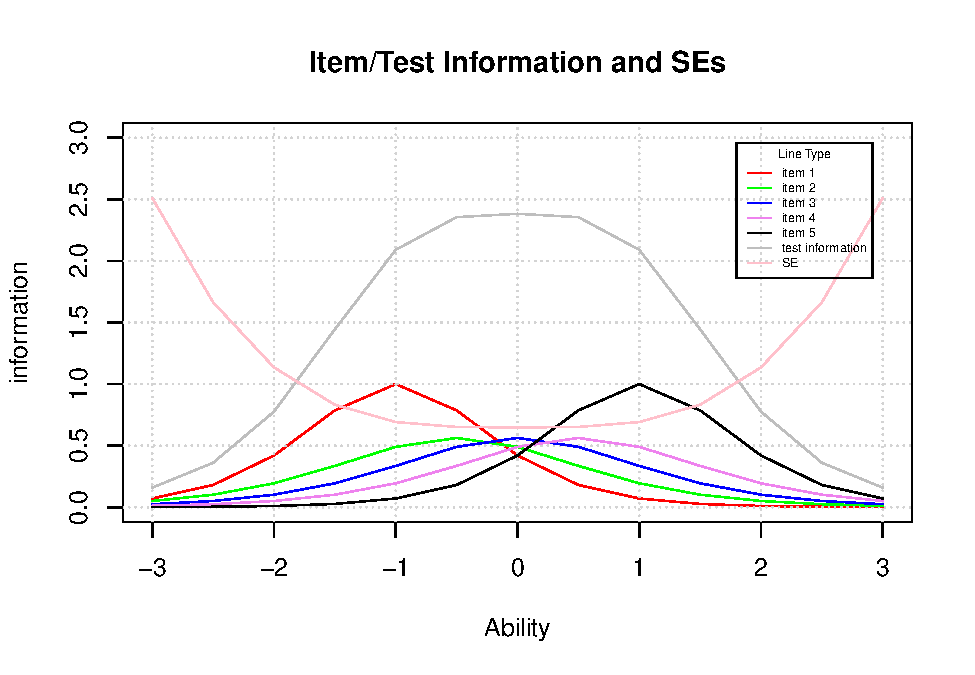
\includegraphics{Assignment_3_files/figure-latex/unnamed-chunk-1-1.pdf}

\end{document}
